The upcoming LHC Run 3 will require more resources than the Worldwide LHC
Computing Grid (WLCG) can provide. Currently, PanDA WMS uses more than
600,000 cores at more than 100 Grid sites, with an aggregated performance of
8 petaFLOPS\@. This capacity will be sufficient for the planned analysis and
data processing, but it will be insufficient for the Monte Carlo production
workflow and any extra activity. To alleviate these challenges, ATLAS is
expanding the current computing model to include additional resources such as
the opportunistic use of supercomputers.

PanDA WMS has been designed to support distributed Grid computing. Executing
ATLAS workloads or workflows involves concurrent and/or sequential runs of
possibly large number of jobs, each requiring minimal, if any parallelization
and no runtime communication. Thus, computing infrastructure like WLCG have
been designed to aggregate large amount of computing resources across
multiple sites. While each site may deploy MPI capabilities, usually these
are not used to perform distributed computations.

Currently, ATLAS workloads do not require fast interconnects or specilized
co-processors, but supercomputers tend not to reach 100\% utilization due to
the scheduling of jobs requiring large amount of resources. This offers the
possibility to execute ATLAS-like workloads on supercomputers to increase
utilization and reducing the waste of available resources.

We developed a single-point solution to better understand the problem space
of enabling a WMS designed for HTC to execute production workflows on
resources designed to support HPC\@. The PanDA team developed a job broker to
support the execution of part of the ATLAS production Monte Carlo workflow on
Titan, a leadership-class supercomputer managed by the Oak Ridge Leadership
Computing Facility (OLCF).

% ---------------------------------------------------------------------------
\subsection{Architectures, Interfaces and Workloads}\label{ssec:panda-titan}

Titan's architecture, configuration and policies poses several challenges to
the deployment of PanDA\@. The default deployment model of PanDA Pilot is
unfeasible on Titan: PanDA Pilot is required to contact the Job Dispatcher of
the PanDA Server to pull jobs to execute, but this is not possible on Titan
because worker nodes do not offer outbound network connectivity. Further,
Titan does not support PanDA's security model based on certificates and
virtual organizations, making PanDA's approach to identity management
unfeasible. While Titan's data transfer nodes (DTNs) offer wide area network
data transfer, an integration with ATLAS DDM is beyond the functional and
administrative scope of the current prototyping phase. Finally, the specific
characteristics of the execution environment, especially the absence of local
storage on the worker nodes and modules tailored to Compute Node Linux,
require re-engineering of ATLAS application frameworks.

Currently, very few HEP applications can benefit from Titan's GPUs but some
computationally-intensive and non memory-intensive tasks of ATLAS workflows
can be off-loaded from the Grid to Titan. Further, when HEP tasks can be
partitioned into independent jobs, Titan worker nodes can be used to execute
up to 16 concurrent payloads, one per each available core. Given these
constraints and challenges, the  Monte Carlo detector simulation task is most
suitable for execution on Titan at the moment. This type of task is mostly
computational-intensive, requiring less than 2GB of RAM at runtime and small
input data. Detector simulation tasks in ATLAS are performed via
AthenaMP~\cite{aad2010atlas}, the ATLAS software framework integrating the
GEANT4 detector simulation toolkit~\cite{agostinelli2003geant4}. These tasks
account for \(\approx\)60\% of all the jobs on WLCG, making them a primary
candidate for offloading.

Detector simulation is part of the ATLAS production Monte Carlo (MC)
workflow~\cite{rimoldi2006atlas}. The MC workflow consists of four main
stages: event generation, detector simulation, digitization, and
reconstruction. Event generation creates sets of particle four-momenta via
different generators, e.g., PYTHIA, HERWIG, and many others. Geant4 simulates
the ATLAS detector and the interaction between the detector and particles.
Each interaction creates a so-called hit and all hits are collected and
passed on for digitalization, where hits are further processed to mimic the
readout of the detector. Finally, reconstruction operates local pattern
recognition, creating high-level objects like particles and jets.

% ---------------------------------------------------------------------------
\subsection{PanDA Broker}\label{ssec:panda_titan}

The lack of wide area network connectivity on Titan's worker nodes is the
most relevant challenge for integrating PanDA WMS and Titan. Without
connectivity, Panda Pilots cannot be scheduled on worker nodes because they
would not be able to communicate with PanDA Server and therefore pull and
execute jobs. This makes impossible to port PanDA Pilot to Titan while
maintaining the defining feature of the pilot abstraction: decoupling
resource acquisition from workload execution via multi-stage scheduling.

The unavailability of pilots is a potential drawback when executing
distributed workloads like MC detector simulation. Pilots are used to
increase the throughput of distributed workloads: while pilots have to wait
in the supercomputer's queue, once scheduled, they can pull and execute jobs
independent from the system's queue. Jobs can be concurrently executed on
every core available to the pilot, and multiple generations of concurrent
executions can be performed until the pilot's walltime is exhausted. This is
particularly relevant for machines like Titan where queue policies privilege
parallel jobs on the base of the number of worker nodes they request: the
higher the number of nodes, the shorter the amount of queue time (modulo
fair-share and allocation policies).

The backfill optimization of Titan's Moab scheduler allows to avoid the
overhead of queue wait times without using pilot
abstraction~\cite{maui_backfill_url}. With this optimization, Moab starts
low-priority jobs when they do not delay higher priority jobs, independent of
whether the low-priority jobs were queued after the high-priority ones.

When the backfill optimization is enabled, users can interrogate Moab about
the number of worker nodes and walltime that would be available to a
low-priority job at that moment in time. If a job is immediately submitted to
Titan with that number of worker nodes and walltime, chances are that Moab
will immediately schedule it, reducing its queue time to a minimum. In this
paper, we call this number of worker nodes and walltime an available
`backfill slot'.

Compared to pilots, backfill has the disadvantage of limiting the amount of
resources that can be requested. Pilots are normal jobs: they can request as
many worker nodes and walltime as a queue can offer. On the contrary, jobs
sized according to an available backfill slot depend on the number of worker
nodes and walltime that cannot be given to any other job at that moment in
time.

At any point in time, the size of an available backfill slot is typically a
small fraction of the total capacity of a resource. Notwithstanding, given
the size of Titan this translates into a substantial capacity. Every year,
about 10\% of Titan's capacity remains unused~\cite{barker2016us},
corresponding to an average of 30,000 unused cores (excluding GPU cores).
This equals to roughly 5\% of the overall capacity of WLCG\@.

Given the communication requirements of PanDA Pilots and the unused capacity
of Titan, PanDA pilot was repurposed to serve as a job broker on the DTN
nodes of Titan (Fig.~\ref{fig:panda_broker}). This prototype called `PanDA
Broker' maintains the core modules of PanDA Pilot and its stand-alone
architecture. This imposes functional trade-offs (e.g., single-threaded
architecture, single MPI PBS script submission) but allows for rapid adoption
and iterative optimization. PanDA Brokers are deployed on DTNs because these
nodes are part of the OLCF infrastructure and can access Titan without RSA
SecureID authentication. DTNs are not part of Titan's worker nodes and,
therefore, are not used to execute Titan's jobs.

Currently, up to 20 PanDA Brokers operate within the existing ATLAS
production software infrastructure, each supporting the execution of MC
detector simulations in 9 steps. Each broker queries the PanDA Server for
ATLAS jobs that have been bound to Titan by JEDI
(Fig.~\ref{fig:panda_broker}:1). Upon receiving jobs descriptions, PanDA
Broker pulls jobs' input files from BNL Data Center to the OLCF Lustre file
system (Fig.~\ref{fig:panda_broker}:2). PanDA Broker queries Titan's Moab
scheduler about the current available backfill slot
(Fig.~\ref{fig:panda_broker}:3) and creates an MPI script, wrapping enough
ATLAS jobs' payload to fit the backfill slot. PanDA Broker submits the MPI
script to the Titan's PBS batch system via RADICAL-SAGA
(Fig.~\ref{fig:panda_broker}:4).

Upon execution on the worker node(s) (Fig.~\ref{fig:panda_broker}:5), the MPI
script initializes and configures the execution environment
(Fig.~\ref{fig:panda_broker}:6), and executes one AthenaMP for each available
work node (Fig.~\ref{fig:panda_broker}:7). AthenaMP retrieves events from
Lustre (Fig.~\ref{fig:panda_broker}:8) and spawns 1 Geant4 event simulation
process on each of the 16 available cores (Fig.~\ref{fig:panda_broker}:9).
Upon completion of each MPI script, PanDA Broker transfer the jobs' output to
BNL (Fig.~\ref{fig:panda_broker}:10), and performs cleanup.

PanDA Broker implementation is resource specific but the ATLAS team has
ported it to other supercomputers, including the HPC2 at the National
Research Center ``Kurchatov Institute''
(NRC-KI)~\cite{belyaev2015integration}, Edison/Cori at the National Energy
Research Scientific Computing Center (NERSC)~\cite{barreiro2016panda}, and
SuperMUC at the Leibniz Supercomputing Centre (LRZ)~\cite{barreiro2016panda}.

\begin{figure}
    \centering
    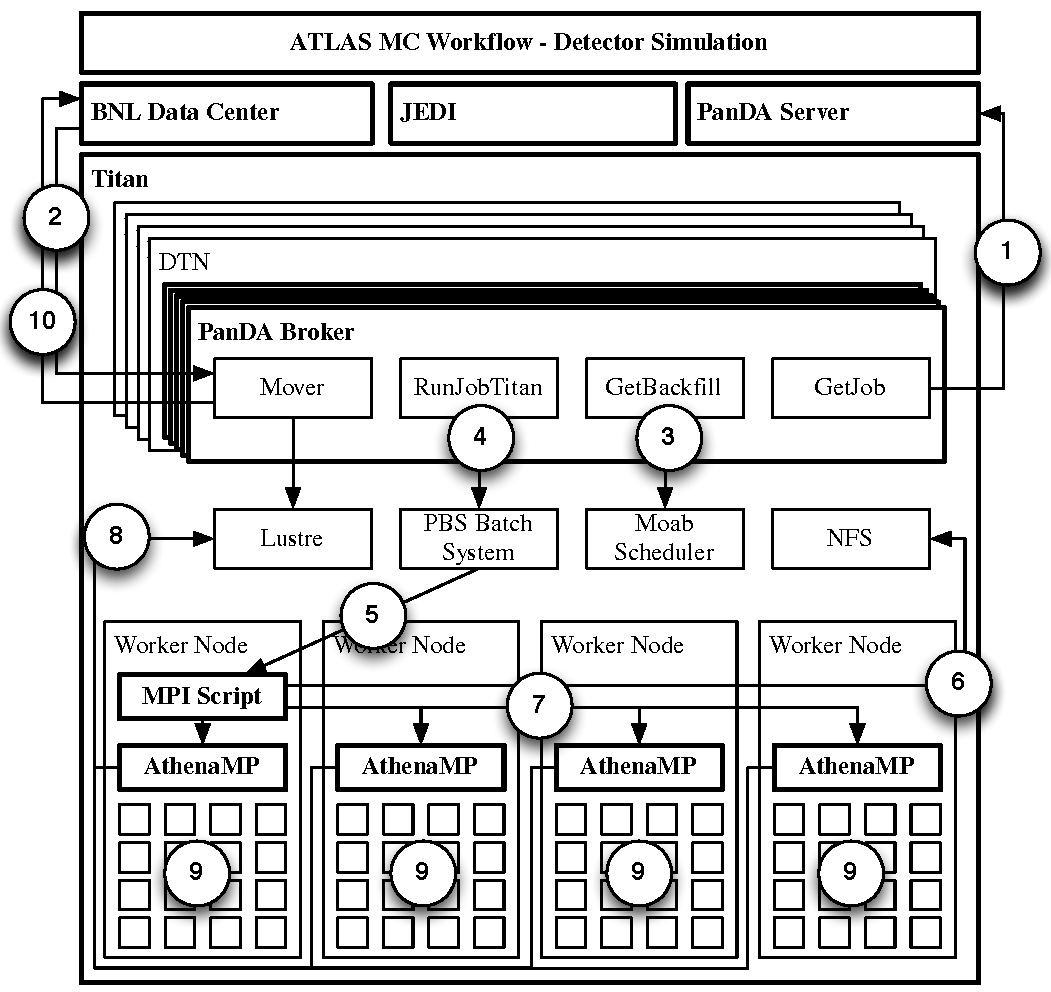
\includegraphics[width=\columnwidth]{panda_broker_architecture.pdf}
    \vspace{-0.3in}
    \caption{PanDA Broker architecture as deployed on Titan. Numbers
    indicates the execution process of a detector simulation job described in
    \S\ref{ssec:panda_titan}.}\label{fig:panda_broker}
\end{figure}
\vspace{-0.04in}
